%% ============================================================
%%  Diseño y validación preliminar de un protocolo de generación
%%  de datos sintéticos de transacciones financieras — Colombia
%%  Trabajo de Grado II · Maestría en IA · Pont. Univ. Javeriana
%%  Plantilla: IEEE Transactions on AI (IEEEtran, journal)
%%
%%  BORRADOR 18-nov-2026. Figuras en figuras/*.pdf (subir esa carpeta
%%  a Overleaf junto a este archivo). Resultados del TSTR (VII.B/C)
%%  PRELIMINARES hasta cerrar WP4/WP8. Texto asistido por IA —
%%  ver docs/reporte/declaracion_uso_ia.md. Reemplazar <...> y % TODO.
%% ============================================================
\documentclass[journal]{IEEEtran}

\usepackage[utf8]{inputenc}
\usepackage[T1]{fontenc}
\usepackage[spanish,es-noshorthands]{babel}
\usepackage{amsmath,amssymb}
\usepackage{booktabs}
\usepackage{array}
\usepackage{url}
\usepackage{graphicx}
\usepackage{hyperref}

\begin{document}

\title{Diseño y validación preliminar de un protocolo de generación de datos sintéticos de transacciones financieras para el contexto colombiano}

\author{Sara Juliana Cárdenas Bohórquez% <-- completar correo institucional en el \thanks
\thanks{Maestría en Inteligencia Artificial, Pontificia Universidad Javeriana, Bogotá, Colombia. Correo: <correo institucional>.}%
\thanks{Directora de tesis: Cecile <apellido>. Manuscrito: 18 de noviembre de 2026.}}

\markboth{Trabajo de Grado II -- Maestría en Inteligencia Artificial, 2026}%
{Cárdenas: Datos sintéticos de transacciones financieras para Colombia}

\maketitle

\begin{abstract}
El acceso a datos transaccionales financieros en Colombia es prácticamente inexistente en el dominio público: su naturaleza privada y sensible —amparada en la Ley 1266 de 2008 (Habeas Data) y la regulación de la Superintendencia Financiera— impide entrenar y validar modelos de clasificación de gastos para la población colombiana. Este trabajo diseña y valida de forma preliminar un protocolo reproducible de generación de datos sintéticos de transacciones (extractos bancarios) calibrado con fuentes abiertas del DANE —la Gran Encuesta Integrada de Hogares (GEIH) 2025 y la Encuesta Nacional de Presupuestos de los Hogares (ENPH) 2016-2017— para Bogotá como caso de estudio. El protocolo adapta el pipeline multi-agente de Pancholi \textit{et al.} incorporando variables ausentes en el modelo de referencia: el estrato socioeconómico y el quintil de ingreso como \textit{priors} bayesianos jerárquicos, y la distribución de medios de pago condicionada a la categoría de gasto. Consta de cuatro etapas: \textit{priors} bayesianos, generador por reglas, refinamiento con CTGAN y validación Train on Synthetic, Test on Real (TSTR). Como contribución metodológica, el pipeline de referencia se reevaluó mediante una ejecución reproducible de su código (etapas 1--4, tres diseños, diez semillas, hasta cinco millones de registros) con criterios prerregistrados: su salida no es mapeable a la taxonomía colombiana (cubre 8 de 16 categorías, con un techo de F1-macro de 0{,}50 por construcción), lo que motiva un protocolo propio; de sus tres limitaciones reportadas, una se refuta, la de medios de pago se corrige y la de sensibilidad al ingreso resulta de su \textit{prompt}, no del modelo generativo. El refinamiento con CTGAN del protocolo propuesto es reproducible bit a bit y, a diferencia del de referencia, conserva la relación ingreso--monto. La validación TSTR contra transacciones reales anotadas de voluntarios bogotanos se reporta como preliminar.
\end{abstract}

\begin{IEEEkeywords}
Datos sintéticos, CTGAN, clasificación de transacciones, TSTR, \textit{priors} bayesianos, informalidad financiera, Colombia.
\end{IEEEkeywords}

\section{Introducción}
\IEEEPARstart{E}{l} desarrollo de sistemas de inteligencia artificial para finanzas personales enfrenta en Colombia una barrera fundamental: la inexistencia de conjuntos de datos públicos de transacciones financieras. A diferencia de contextos como el estadounidense, donde existen bases abiertas derivadas de encuestas de consumidores y registros de pagos, en Colombia los datos transaccionales son estrictamente privados y están bajo el resguardo de entidades sujetas a la Ley 1266 de 2008 (Habeas Data) y a la Superintendencia Financiera. Esta restricción no es técnica sino regulatoria y de privacidad: no se resuelve con más cómputo ni mejores algoritmos.

La brecha impide entrenar, validar y replicar modelos de clasificación de gastos, detección de patrones de ahorro o asesoría financiera para la población colombiana. El problema se agrava por la estructura del país: según el Banco de la República, el efectivo es el instrumento más usado en los pagos habituales (77{,}8\,\% de las transacciones en su encuesta de 2024 \cite{banrep2024}), y la tenencia de tarjeta de crédito es minoritaria (7{,}2\,\% de los hogares \cite{rif2024}). Estas características hacen inviable transferir directamente modelos entrenados con datos de economías formalizadas.

Pancholi \textit{et al.} \cite{pancholi2026} propusieron un sistema integral de finanzas personales basado en IA que incluye un generador de datos sintéticos, un clasificador de gastos y un asesor de inversión. Aunque su contribución metodológica es relevante, el sistema fue diseñado y validado exclusivamente con datos demográficos del American Community Survey de Washington D.C. y comercios de Yelp y de esa ciudad. Como parte de este trabajo, el pipeline se ejecutó y se reevaluó de forma reproducible (Sección~\ref{sec:pancholi}); sus tres limitaciones reportadas —insensibilidad al ingreso, sesgo de categorías hacia el ocio y asignación monolítica del medio de pago— se contrastan con criterios prerregistrados en lugar de darse por sentadas.

Ante esta situación, se propone un protocolo de generación de datos sintéticos de transacciones calibrado para el contexto colombiano, con \textbf{Bogotá urbana como caso de estudio} (el dominio donde se recolecta el conjunto real de validación, lo que exige calibrar y evaluar en el mismo dominio). El protocolo usa como insumos la GEIH 2025 y la ENPH 2016-2017 del DANE para construir \textit{priors} bayesianos que reflejen la estructura demográfica y de gasto real, y su utilidad se valida mediante el paradigma Train on Synthetic, Test on Real (TSTR) \cite{esteban2017}. Las contribuciones son: (i) un protocolo replicable para economías de alta informalidad; (ii) un primer conjunto sintético público de transacciones colombianas; (iii) una reevaluación reproducible y prerregistrada del pipeline de referencia; y (iv) evidencia, vía TSTR, del valor de la contextualización.

\section{Trabajo relacionado}
\subsection{Generación de datos sintéticos financieros}
Lopez-Rojas \textit{et al.} \cite{paysim2016} desarrollaron PaySim, un simulador de transacciones móviles basado en agentes y calibrado con datos reales anonimizados, orientado a detección de fraude; no modela categorías de gasto ni perfiles demográficos, y opera sobre transferencias y pagos sin considerar el efectivo. Xu \textit{et al.} \cite{ctgan2019} propusieron el Conditional Tabular GAN (CTGAN), que extiende las GAN a datos tabulares con tipos mixtos, distribuciones no gaussianas y desbalance de clases, mediante normalización específica por modo y un generador condicional; es el componente del módulo de refinamiento de este trabajo. Altman \textit{et al.} \cite{altman2023} aportaron un generador con \textit{ground truth} completo para modelos de lavado de activos. Hounwanou \textit{et al.} \cite{hounwanou2025} compararon modelos generativos para datos financieros. Karst \textit{et al.} \cite{karst2024} compararon CTGAN, DGAN, FinDiff y TVAE sobre datos bancarios, hallando en CTGAN el mejor equilibrio entre fidelidad distribucional y capacidad de síntesis.

\subsection{Clasificación automática de transacciones}
La clasificación de transacciones es un problema de clasificación de texto con descripciones cortas, vocabulario de dominio y alto desbalance de clases. Pancholi \textit{et al.} \cite{pancholi2026} evaluaron regresión logística con TF-IDF, LSTM, BERT \textit{fine-tuneado} y LLaMA~3 en modo \textit{few-shot}, con mejor desempeño de LLaMA~3, pero exclusivamente sobre transacciones en inglés de Washington D.C. En el contexto colombiano la investigación es escasa y sin datasets públicos, lo que justifica la contribución de datos sintéticos abiertos.

\subsection{Train on Synthetic, Test on Real (TSTR)}
TSTR fue formalizado por Esteban \textit{et al.} \cite{esteban2017}: se entrena sobre datos sintéticos y se evalúa sobre datos reales no vistos, midiendo la utilidad práctica más allá de la fidelidad distribucional. Su aplicación a finanzas personales colombianas, donde los datos reales son escasos \emph{por diseño}, es una de las contribuciones metodológicas de este trabajo.

\section{Planteamiento del problema e hipótesis}
El desarrollo de clasificadores de gastos para usuarios colombianos enfrenta una contradicción estructural: entrenar un modelo requiere transacciones etiquetadas, pero esos datos son privados por diseño y no existen en el dominio público. La restricción es regulatoria, no técnica. Usar datos sintéticos de pipelines calibrados en otros países no es viable sin adaptación: la reevaluación reproducible del pipeline de referencia (Sección~\ref{sec:pancholi}) muestra que no reproduce la relación ingreso--gasto ni la estructura de medios de pago colombiana.

\textbf{Pregunta.} ¿Puede un protocolo calibrado con fuentes colombianas (GEIH 2025 y ENPH 2016-2017) producir transacciones suficientemente realistas para entrenar un clasificador de gastos que funcione sobre transacciones reales de usuarios bogotanos, validado mediante TSTR?

\textbf{Hipótesis.} Un pipeline que incorpore el estrato socioeconómico y el quintil de ingreso como \textit{priors} bayesianos, y la distribución de medios de pago condicionada a la categoría de gasto observada en Colombia, producirá datos sintéticos con utilidad de entrenamiento suficiente —medida por F1-macro en TSTR sobre transacciones reales bogotanas— para un clasificador de gastos funcional. La contextualización no es opcional: el pipeline de referencia no cubre, por construcción, el espacio de categorías colombiano (Sección~\ref{sec:pancholi}), de modo que la comparación pertinente es la ganancia que aporta la capa estructural propia (ablación generador por reglas frente a CTGAN), no un F1 cabeza a cabeza con un pipeline no mapeable. Bajo la arquitectura de dos capas (Sección~\ref{sec:metodo}), la ENPH calibra la capa interna de gasto del hogar; la participación de billeteras y transferencias en la capa observable se introduce mediante una regla de migración parametrizada por escenarios (10/20/35\,\%), dado que la ENPH 2016-2017 no registra esos instrumentos, y el TSTR se reporta bajo los tres escenarios.

\section{Datos y metodología}
\label{sec:metodo}
\subsection{Fuentes de datos y dominio}
Se usan dos fuentes abiertas del DANE con una regla de calibración explícita: \textbf{la ENPH aporta ingreso (\texttt{ICGU}) y gasto; la GEIH aporta la estructura demográfica y laboral}; el ingreso laboral individual (\texttt{INGLABO}) es solo descriptivo por su amontonamiento en valores redondos. La GEIH 2025 (12 meses apilados) aporta estrato, posición ocupacional, formalidad y tenencia de productos financieros (muestra de Bogotá: 9\,733 hogares y 13\,552 ocupados); la ENPH 2016-2017 aporta ingreso del hogar, gasto por categoría y forma de pago (\texttt{NC2R}, \texttt{P438}) (muestra: 3\,918 hogares). El dominio es Bogotá urbana (\texttt{AREA}=11; la llave de hogar en ENPH es \texttt{DIRECTORIO}). Todo cálculo usa factores de expansión (\texttt{FEX\_C18/FEX\_C12} en GEIH, \texttt{FEX\_C} en ENPH), los 112 archivos del DANE se verifican por SHA-256 y ninguna cifra se escribe a mano: toda cifra se deriva por código y queda en el repositorio.

\subsection{Hallazgos descriptivos que calibran el protocolo}
La Fig.~\ref{fig:estrato} muestra la distribución de estrato en ambas encuestas, que coinciden razonablemente pese a los nueve años de diferencia, lo que respalda usar la GEIH como estructura. La forma de pago principal en gastos frecuentes (\texttt{NC2R}, $n{=}3\,517$) es efectivo 97{,}0\,\%, débito 2{,}0\,\%, crédito 0{,}5\,\% y otras 0{,}5\,\% (no respuesta 11{,}4\,\%). Ahora bien, el medio de pago no es uniforme: varía con la categoría de gasto (Fig.~\ref{fig:medio}). El efectivo supera el 85\,\% en 22 de 29 subcapítulos, pero la tarjeta de crédito asciende donde el gasto es grande y planeado (electrodomésticos y muebles, 28{,}0\,\%; transporte, 22{,}4\,\%). Esta matriz categoría $\times$ medio es uno de los insumos que diferencian el protocolo del modelo de referencia, que asigna un único medio. En el mercado laboral, el 58{,}9\,\% son empleados particulares y el 30{,}5\,\% trabaja por cuenta propia, lo que define cómo el generador modela el ingreso (nómina vs. depósitos irregulares). El 93{,}47\,\% de los hogares tiene al menos un producto financiero, cifra que fija el universo bancarizado del generador.

\begin{figure}[!t]
\centering
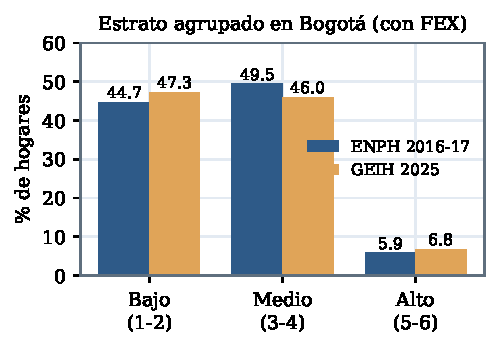
\includegraphics[width=0.82\columnwidth]{figuras/fig_estrato.pdf}
\caption{Distribución de estrato agrupado en Bogotá en ambas encuestas, con factores de expansión. La coincidencia respalda usar la GEIH 2025 como estructura demográfica.}
\label{fig:estrato}
\end{figure}

\begin{figure}[!t]
\centering
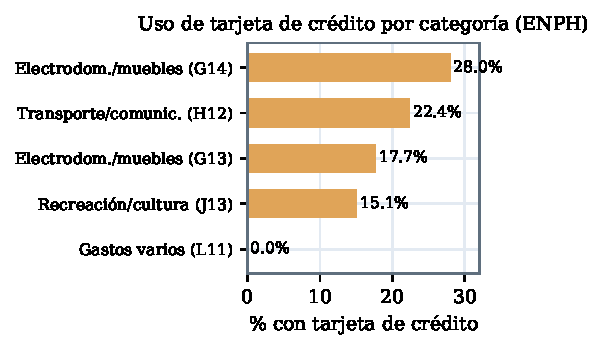
\includegraphics[width=0.92\columnwidth]{figuras/fig_medio_categoria.pdf}
\caption{Uso de tarjeta de crédito por subcapítulo de gasto (ENPH, con FEX). El medio de pago depende de la categoría: el generador lo condiciona a ella en vez de asignar un medio único.}
\label{fig:medio}
\end{figure}

\subsection{Decisiones de diseño}
El protocolo documenta quince decisiones de diseño con su justificación. Las centrales: dominio Bogotá urbana; «ENPH calibra, GEIH estructura»; estrato agrupado en 3 $\times$ quintil de ingreso en 5 (quince celdas); encogimiento jerárquico para las celdas ralas; la arquitectura de dos capas (el generador emite extractos bancarios, no el gasto total del hogar); y la separación estricta entre datos reales y calibración —los datos reales solo evalúan, nunca calibran—, que evita contaminar el TSTR.

\subsection{Las cuatro etapas}
\textbf{Etapa 1 — \textit{Priors} bayesianos.} Para cada una de las quince celdas (estrato $\times$ quintil) se estima la distribución categórica de gasto, forma y medio de pago, y ocupación, como media posterior de un Dirichlet jerárquico:
\begin{equation}
\pi_{\text{post}} = \frac{n\,\hat{p} + \kappa\,\pi_{\text{padre}}}{n + \kappa},
\label{eq:prior}
\end{equation}
donde $\hat{p}$ son las proporciones ponderadas por FEX de la celda, $n$ es el tamaño efectivo de Kish $(\sum w)^2/\sum w^2$ —que corrige por pesos de expansión desiguales—, $\pi_{\text{padre}}$ es la distribución del nivel urbano nacional \emph{recalibrada} para que su media ponderada coincida con el marginal de Bogotá (aporta forma entre celdas, no nivel), y $\kappa$ es la concentración, estimada por máxima verosimilitud marginal (Dirichlet-multinomial), no elegida a mano. Una celda se encoge hacia el padre cuando $n_{\text{ef}} < \hat{\kappa}$; con la agrupación en quince celdas, solo cuatro (estrato alto en los quintiles bajos) resultan ralas.

\textbf{Etapa 2 — Generador por reglas.} Muestrea perfiles de hogares bancarizados a partir de los \textit{priors} y emite el extracto bancario en dos capas: una capa interna simula el gasto completo del hogar calibrado con la ENPH, y una capa emitida contiene lo que vería un banco —compras (con el medio condicionado a la categoría), retiros, nómina, transferencias P2P, recargas y pagos recurrentes—. El efectivo de la capa interna se convierte en retiros periódicos. Los montos de la ENPH se deflactan a pesos de 2025 con el índice total del IPC nacional del DANE, aplicando a cada hogar el factor de su mes de recolección (entre 1{,}56 y 1{,}62). La validación interna confirma la calibración: el gasto sobre ingreso por hogar tiene mediana 0{,}93 (ENPH observada 0{,}94) y el efectivo simulado se retira casi en su totalidad.

\textbf{Etapa 3 — Refinamiento con CTGAN} (SDV): aprende correlaciones de alto orden entre los campos estructurados del extracto, con pre-registro de columnas, métricas y reglas duras (Sección~\ref{sec:resultados}).

\textbf{Etapa 4 — Validación TSTR:} entrenar clasificadores sobre sintético y evaluarlos sobre el conjunto real anotado de Bogotá (Sección~\ref{sec:exp}).

\section{Reevaluación del pipeline de referencia}
\label{sec:pancholi}
Las tres limitaciones que se atribuían al pipeline de referencia se reevaluaron \emph{ejecutando su propio código} (clon con \textit{commit} fijo, con sus dependencias), no repitiendo las afirmaciones. Se corrieron las etapas 1--3 en tres diseños —A, rejilla de ingreso que fija hogar y ZIP para aislar su efecto; B, réplica literal de su sintetizador con sus 155 clientes; C, su etapa~1 reentrenada seguida de las etapas 2--3— con diez semillas por diseño (salvo C), hasta cinco millones de registros, intervalos de confianza por \textit{bootstrap} entre semillas y criterios de evaluación fijados por escrito antes de correr. La corrida de la semilla de referencia se repitió con resultado idéntico. La \textbf{etapa~4} (enriquecimiento con un modelo de lenguaje) se corrió después con un modelo sustituto (\texttt{gpt-oss-120b}, porque Groq retiró el modelo original el 16-ago-2026) en una sola corrida, como evidencia indicativa. Las cifras del informe de avance inicial (cinco perfiles, 149 transacciones, «USD~12», 100\,\% tarjeta) provenían de su aplicación web —no del pipeline del paper— y se retiran.

\begin{figure}[!t]
\centering
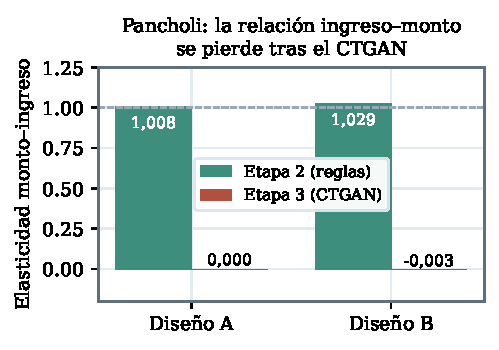
\includegraphics[width=0.82\columnwidth]{figuras/fig_pancholi_elasticidad.pdf}
\caption{Elasticidad monto--ingreso en el pipeline de referencia. La etapa de reglas la conserva ($\approx 1$); la salida del CTGAN la colapsa a $\approx 0$ porque el ingreso no es una de sus columnas de entrenamiento. Media de diez semillas.}
\label{fig:pancholi}
\end{figure}

Los resultados (Tabla~\ref{tab:pancholi}, Fig.~\ref{fig:pancholi}): la etapa de reglas respeta la relación ingreso--monto (elasticidad $\approx 1$), pero la salida final del CTGAN la pierde (elasticidad $\approx 0$, con intervalo que incluye el cero), porque el ingreso no es una columna de su entrenamiento. Prerregistrar los criterios es lo que da credibilidad a la reevaluación: no se ajustó la definición para obtener un resultado. La conclusión que sostiene el protocolo es que el pipeline de referencia no reproduce ni la relación ingreso--gasto ni la estructura de medios de pago colombiana; adaptarlo no es opcional. Más aún, su salida \textbf{no es mapeable} a la taxonomía colombiana: solo emite compras y alcanza 8 de las 16 categorías, de modo que cualquier clasificador entrenado con ella tiene un \textbf{techo de F1-macro de 0{,}50} por construcción (falta el 42\,\% de las transacciones observables: ingreso, retiro, movimiento propio, P2P y otras). Esa no-transferibilidad es, en sí misma, el resultado que motiva un protocolo propio.

\begin{table}[!t]
\caption{Reevaluación de las hipótesis sobre el pipeline de referencia (etapas 1--4)}
\label{tab:pancholi}
\centering
\footnotesize
\begin{tabular}{p{0.8cm}p{2.1cm}p{4.2cm}}
\toprule
Hip. & Enunciado & Veredicto tras la ejecución \\
\midrule
H-P1 & Insensibilidad al ingreso & Las reglas conservan la relación (elasticidad 1{,}008) y la etapa~4 responde al ingreso (0{,}79) solo porque su \textit{prompt} inyecta un rango de gasto derivado del ingreso; el CTGAN la pierde ($-0{,}003$). El CTGAN propio sí la conserva ($r\approx1{,}37$). \\
H-P2 & Dominio de ocio & \textbf{Refutada} con la definición prerregistrada (entretenimiento 13{,}0\,\% vs. alimentos 14{,}8\,\%); confirmada solo si el hospedaje cuenta como ocio. \\
H-P3 & 100\,\% tarjeta & No emite retiros, transferencias ni billetera (0 de 5\,M). La etapa~4 \textbf{sí se ejecutó}: domina la tarjeta (89\,\% crédito) pero \textbf{no es 100\,\%} (efectivo/billetera/transferencia 0 de 300). \\
\bottomrule
\end{tabular}
\end{table}

\section{Diseño experimental}
\label{sec:exp}
\subsection{Dataset sintético}
La corrida de referencia del generador produce, para 1\,000 perfiles $\times$ 3 meses (semilla 42), 448\,383 filas internas de las cuales 122\,211 se emiten. A diferencia del pipeline de referencia —que emite un solo tipo de registro—, el extracto sintético contiene ocho tipos de movimiento (Fig.~\ref{fig:emitidas}), incluidos casi 19\,000 retiros de efectivo: así entra el efectivo al extracto. El monto mediano emitido es \$24.100 y el percentil 99, \$2{,}9 millones. Sobre este conjunto se entrena el CTGAN de la Etapa~3.

\begin{figure}[!t]
\centering
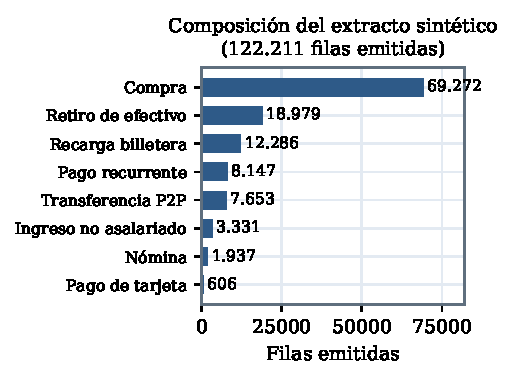
\includegraphics[width=0.92\columnwidth]{figuras/fig_emitidas.pdf}
\caption{Composición del extracto sintético por tipo de movimiento (capa emitida, 122\,211 filas). El pipeline de referencia solo emite compras; aquí el efectivo aparece como retiros.}
\label{fig:emitidas}
\end{figure}

\subsection{Conjunto real de validación}
La validación usa extractos de 20 voluntarios de Bogotá (muestra por conveniencia; conjunto de validación, no representativo), de billeteras (Nequi, Daviplata) o bancarios, anonimizados según protocolo y etiquetados por dos anotadores con la taxonomía, con concordancia inter-anotador (Cohen's Kappa). Estado: aval de ética resuelto; ingesta, anonimización y anotación en curso.

\subsection{Protocolo TSTR y clasificadores}
Se entrenan tres clasificadores sobre el sintético: regresión logística con TF-IDF (baseline), BETO \textit{fine-tuneado} y LLaMA~3 \textit{few-shot}. Métricas: F1-macro (con regla de soporte $\ge 10$ por clase), Cohen's Kappa y AUC. Dado que la descripción textual se genera por plantillas condicionadas a la categoría, un clasificador de texto mediría las plantillas y no el aporte del CTGAN; por eso se incluye un \textbf{brazo de control con solo campos estructurados} que aísla la contribución del refinamiento generativo. \textbf{Comparación con el pipeline de referencia:} la comparación justa no es contra el desempeño que los autores reportan (medido sobre datos en inglés de otra ciudad, con otras categorías), sino entrenar un clasificador sobre la salida de \emph{su} pipeline y evaluarlo sobre el \emph{mismo} conjunto real de Bogotá; el desempeño reportado por los autores se cita como contexto, no como un número directamente comparable.

\section{Resultados}
\label{sec:resultados}
\subsection{Fidelidad del dataset sintético}
Corrida oficial: 300 épocas en CPU, semilla 42 (SDV 2.2.0, ctgan 0.13.0), con reproducibilidad \textbf{bit a bit confirmada} (SHA-256 idéntico en dos entrenamientos independientes). Train = 96\,386 filas (80\,\% de perfiles); holdout = 25\,825. La Tabla~\ref{tab:fidelidad} resume la calidad SDV frente al piso (marginales independientes) y el techo (train vs. holdout).

\begin{table}[!t]
\caption{Fidelidad del dataset sintético v1 (SDV QualityReport)}
\label{tab:fidelidad}
\centering
\begin{tabular}{lccc}
\toprule
Métrica & Piso & CTGAN v1 & Techo \\
\midrule
Overall            & 0{,}830 & 0{,}931 & 0{,}974 \\
Column Shapes      & 0{,}980 & 0{,}935 & 0{,}980 \\
Column Pair Trends & 0{,}680 & 0{,}927 & 0{,}968 \\
\bottomrule
\end{tabular}
\end{table}

En dependencias (Column Pair Trends) el CTGAN recupera el 85{,}7\,\% de la distancia piso$\rightarrow$techo, que es su aporte sobre un muestreo trivial; en marginales (Column Shapes) queda por debajo del piso, que las clava por construcción. La elasticidad monto--ingreso da veredicto \textbf{CONSERVA}: train $\hat{e}=0{,}331$ [0{,}267; 0{,}388] frente a CTGAN $\hat{e}=0{,}452$ [0{,}441; 0{,}463], razón $r=1{,}37$ (incluso amplifica, $r>1$), en contraste con el $-0{,}003$ del pipeline de referencia (Fig.~\ref{fig:pancholi}). La tasa de rechazo por reglas duras fue 14{,}78\,\%, por encima del tope prerregistrado del 10\,\% (resultado de fidelidad negativo, reportado): el grueso (10{,}78\,\%) son pares categoría--subcategoría fuera de la taxonomía, lo que indica que el CTGAN plano no captura bien la jerarquía categórica.

\subsection{Validación TSTR}
\emph{[Preliminar, WP8.]} F1-macro por clasificador, matriz de confusión por categoría y Kappa, pendientes de la anotación del conjunto real.

\subsection{Comparación con el pipeline de referencia}
El pipeline de referencia no es mapeable a la taxonomía colombiana (Sección~\ref{sec:pancholi}): su salida cubre 8 de 16 categorías, con un techo de F1-macro de 0{,}50 por construcción, así que \textbf{no entra como fila comparable} en la tabla TSTR. La comparación es estructural —la no-transferibilidad del pipeline de referencia frente a la cobertura completa del protocolo propio—, no un F1 medido cabeza a cabeza; el desempeño que los autores reportan se cita solo como contexto. La tabla TSTR contrasta las dos variantes propias (generador por reglas vs. generador con CTGAN, ablación de la Etapa~3) sobre el mismo conjunto real. \emph{[Preliminar, WP8.]}

\section{Discusión y limitaciones}
El aporte disponible es doble: una base empírica reconstruida y verificable de Bogotá con un protocolo de generación de \textit{priors} jerárquicos y medios de pago condicionados a la categoría; y una reevaluación reproducible y prerregistrada del pipeline de referencia. El refinamiento con CTGAN, además de reproducible bit a bit, conserva la relación ingreso--monto que el pipeline de referencia pierde. La validación TSTR es preliminar; acota, no cierra, la hipótesis.

Limitaciones principales: los archivos públicos no traen segmento ni UPM, por lo que no se reportan intervalos de confianza de diseño sobre cifras del DANE; la ENPH es de 2016-2017 y no registra billeteras ni transferencias, que se introducen por una regla de migración por escenarios sin ancla verificada; los extractos no ven el efectivo (un retiro es una fila, no quince compras), por lo que el TSTR se evalúa sobre el universo bancarizado; los 20 voluntarios son una muestra por conveniencia. La reevaluación del pipeline de referencia ejecutó sus etapas 1--4 (la etapa~4 con un modelo sustituto en una sola corrida, como evidencia indicativa; la etapa~5 de asesoría de inversión queda fuera de alcance). Dos límites propios del CTGAN: genera un 10{,}78\,\% de pares categoría--subcategoría inexistentes (no modela bien la jerarquía categórica), y amplifica la elasticidad por encima del \textit{train} (posible sobre-ajuste de la correlación ingreso--monto). Finalmente, el texto sintético se genera por plantillas, más limpias que un extracto real, por lo que el TSTR será un techo optimista; y el CTGAN se entrena sobre la capa emitida, que ya es sintética, de modo que su fidelidad es a la salida de las reglas, no a la realidad colombiana —la prueba frente a la realidad es el TSTR—.

\section{Conclusiones y trabajo futuro}
El trabajo entrega un protocolo reproducible para generar extractos bancarios sintéticos calibrado con microdatos del DANE para Bogotá, con \textit{priors} bayesianos jerárquicos por estrato y quintil, medios de pago condicionados a la categoría, y una reevaluación prerregistrada del pipeline de referencia cuya principal diferencia —la conservación de la relación ingreso--monto— se verifica en el refinamiento propio. Trabajo futuro: cerrar la validación TSTR con el conjunto real anotado; extender a otras ciudades; anclar la participación de medios digitales con una fuente primaria; modelar explícitamente la jerarquía categórica en el CTGAN; y reemplazar la biblioteca curada de comercios por una capa empírica.

\section*{Declaración de uso de herramientas de IA}
Este trabajo se apoyó en asistentes de IA para programación, depuración y redacción asistida, bajo la dirección de la autora, quien definió la metodología, tomó las decisiones de diseño, ejecutó el pipeline sobre los microdatos y verificó los resultados. El detalle por fase está en \texttt{docs/reporte/declaracion\_uso\_ia.md}. La reproducibilidad del repositorio (pruebas automatizadas, SHA-256, semillas fijas, cifras generadas por código) permite auditar cada resultado de forma independiente.

\begin{thebibliography}{11}
\bibitem{pancholi2026} S.~Pancholi, A.~Jaglan, H.~Makadia, P.~Doshi, and M.~Jafari, ``An end-to-end multi-agent AI system for personal finance: synthetic data generation, budget optimization, and investment advisory,'' \textit{Neural Computing and Applications}, vol.~38, 2026, doi: 10.1007/s00521-025-11749-7.
\bibitem{banrep2024} Banco de la República de Colombia, ``Resultados de la encuesta de percepción sobre el uso de los instrumentos para los pagos habituales en Colombia 2024,'' Bogotá, 2024.
\bibitem{geih2025} DANE, ``Gran Encuesta Integrada de Hogares --- GEIH 2025,'' Bogotá, 2025. [Online]. Available: \url{https://microdatos.dane.gov.co/index.php/catalog/853}
\bibitem{enph2017} DANE, ``Encuesta Nacional de Presupuestos de los Hogares --- ENPH 2016-2017,'' Bogotá, 2017. [Online]. Available: \url{https://microdatos.dane.gov.co/index.php/catalog/566}
\bibitem{esteban2017} C.~Esteban, S.~L.~Hyland, and G.~Rätsch, ``Real-valued (medical) time series generation with recurrent conditional GANs,'' \textit{arXiv:1706.02633}, 2017.
\bibitem{paysim2016} E.~A.~Lopez-Rojas, A.~Elmir, and S.~Axelsson, ``PaySim: A financial mobile money simulator for fraud detection,'' in \textit{Proc. 28th European Modeling and Simulation Symp. (EMSS)}, Larnaca, Cyprus, 2016.
\bibitem{ctgan2019} L.~Xu, M.~Skoularidou, A.~Cuesta-Infante, and K.~Veeramachaneni, ``Modeling tabular data using conditional GAN,'' in \textit{Advances in Neural Information Processing Systems (NeurIPS)}, vol.~32, 2019.
\bibitem{altman2023} E.~Altman \textit{et al.}, ``Realistic synthetic financial transactions for anti-money laundering models,'' in \textit{NeurIPS Datasets and Benchmarks Track}, 2023, \textit{arXiv:2306.16424}.
\bibitem{hounwanou2025} C.~D.~Hounwanou, P.~Ntakirutimana, and Y.~U.~Gaba, ``Evaluating generative models for synthetic financial data,'' \textit{arXiv:2512.21791}, 2025.
\bibitem{karst2024} N.~Karst \textit{et al.}, ``Generative AI for banks: Benchmarks and algorithms for synthetic financial transaction data,'' \textit{arXiv:2412.14730}, 2024.
\bibitem{rif2024} Banca de las Oportunidades y Superintendencia Financiera de Colombia, ``Reporte de Inclusión Financiera 2024,'' Bogotá, 2024.
\end{thebibliography}

\end{document}
